\documentclass{article}
\usepackage{hyperref}
\usepackage{graphicx}
\graphicspath{{./Images/}}
\usepackage[margin=1.25in]{geometry}
\title{\textbf{Balancing Weighted Partial Ballots (BWPB)}\\ \large  Tabulation Manual for the 3rd Annual Richard Calkins Invitational}
\author{Ray Barr\footnote{Ray is the former tournament director of the Richard Calkins Invitational, the former president of Drake Mock Trial, and a current student at the University of Minnesota School of Law.  Comments and questions may be directed to \href{mailto:allencbarr@gmail.com}{allencbarr@gmail.com}.  While the methods and policies described herein are the official tabulation policies of the Richard Calkins Invitational, all accompanying explanations, opinions, and commentary are solely those of the author and do not represent the official views of Drake Mock Trial  or Drake University.  This work is licensed under the Creative Commons Attribution-ShareAlike 4.0 International License. To view a copy of this license, visit \url{http://creativecommons.org/licenses/by-sa/4.0/} or send a letter to Creative Commons, 444 Castro Street, Suite 900, Mountain View, California, 94041, USA.}}
\begin{document}
\maketitle
\begin{abstract}
The primary purpose of this document is to describe the tabulation procedures that will be used at the 2014 Richard Calkins Invitational, as they are not those found in the standard AMTA Tabulation Manual.  Instead, the Richard Calkins Invitational will be using a method of tabulation known as Balancing Weighted Partial Ballots (BWPB).  This method takes aspects of weighted ballot systems that have been used at other invitational tournaments and makes two additions/modifications.  First, the curve defining the amount of partial ballots won is modified to better achieve the goals it serves.  Second, a means of correcting for side-bias is introduced, in the form of varying what constitutes a ``quality win'' for each side depending on the number of plaintiff and defense ballots won.  This manual attempts to justify the theory behind these components of BWPB and explain how they will be implemented at the Richard Calkins Invitational this year.
\end{abstract}
\section{The Problem With Standard Tabulation}
BWPB has the potential to be considered a solution in need of a problem.  Approximately 80 tournaments each year use standard AMTA tabulation (SAT), and aside from perhaps the occasional grumble on Perjuries or Mock Trial Confessions, no one finds the system of tabulation seriously flawed at those tournaments.  Why then, use another system of tabulation?

The answer lies in what the different methods of tabulation focus on as being the best indicator of a superior team.  SAT focuses solely on ballots won.  If team 1985 has won more ballots than team 1986, then team 1985 is considered the better team, regardless of the point differentials on those ballots or the strength of their opponents; a team that goes $+1$ on every ballot is considered a better team than a team that goes $+10$ on $7$ ballots and $-1$ on the eighth.  BWPB, on the other hand, considers both of these factors in its ranking of teams.

Reasonable minds may differ as to what factors should be considered in determining a superior team\footnote{It would be \textit{very} interesting to consider how scoring would differ if something akin to a sportsmanship score or SPAMTA was used in team rankings.}, the argument that a team that persuades the most judges is the best team being the argument most commonly given in favor of SAT.  Certainly, this position is not unreasonable, however, using SAT may also lead to several consequences typically considered undesirable.  First, teams are encouraged to perform \textit{just well enough} to win the ballot, \textbf{not} to the best of their ability, as a higher point differential (PD) leads to facing ``harder'' opponents, for which there is no reward as opposed to facing ``easier'' opponents.  Second, the idiosyncrasies of a judge may cause them to score one part higher than all other, qualitatively similar parts.  This costs one of the (otherwise similar) teams the entirety of the ballot.  Third, SAT does not account for case balance; winning on the plaintiff and winning on the defense are both achieved by having $1$ more point than your opponent, regardless of any case imbalances that may exist.  For these (and other) reasons, BWPB provides a welcome alternative to SAT.
\section{Balancing Weighted Partial Ballots}
In response to these concerns, several tournaments have used a method of tabulation known as ``Weighted Partial Ballots''.  Various tournaments have reported WPB statistics, and the Yale Invitational used them for tabulation in 2013.  To my knowledge, however, no tournament has incorporated the balancing term presented here, nor a ``victory curve'' identical to the one justified herein.  BWPB incorporate three key things:  assigning partial wins to teams based on individual ballot PD, balancing what constitutes a complete win based on case balance at the tournament, and weighting won ballots to account for opponent strength.
\subsection{Partial Ballots}
The first aspect captured by BWPB not captured by SAT is the point differential of a round.  While SAT tabulation assigns a complete win or loss on the basis of a PD of only $+1$ or $-1$, both WPB and BWPB use a gradual scale, assigning fractions of the ballot to each team based on the PD (hence the word ``partial'' ballot).  In order to earn a complete win, a team must win the ballot by at least certain point differential, referred to as a ``quality win'' (QW).  Tournaments that have used partial ballots in the past have typically defined $QW=14$.  Any PD above the QW does not increase further the amount of ballots won, rather the winning team earns a complete ballot and the losing team earns no ballot.  Should the PD be less than the QW, however, the teams are allotted a faction of the ballot, based on a gradual curve within $-QW<PD<QW$.  There are two defining components of this gradual scale:  the form of the equation (affecting the shape of the curve), and the quality win (affecting where the endpoints of the scale occur).  The shape of the curve is discussed in the remainder of this section, while selecting the QW is discussed in section \ref{balancingBallots}.

There are an infinite number of functions that could map a PD between $-QW$ and $QW$ onto a fraction of a ballot.  As shown in Figure \ref{ballotCurves}
\begin{figure}[h]
\centering
\caption{Various Possible Quality Win Curves}
\label{ballotCurves}
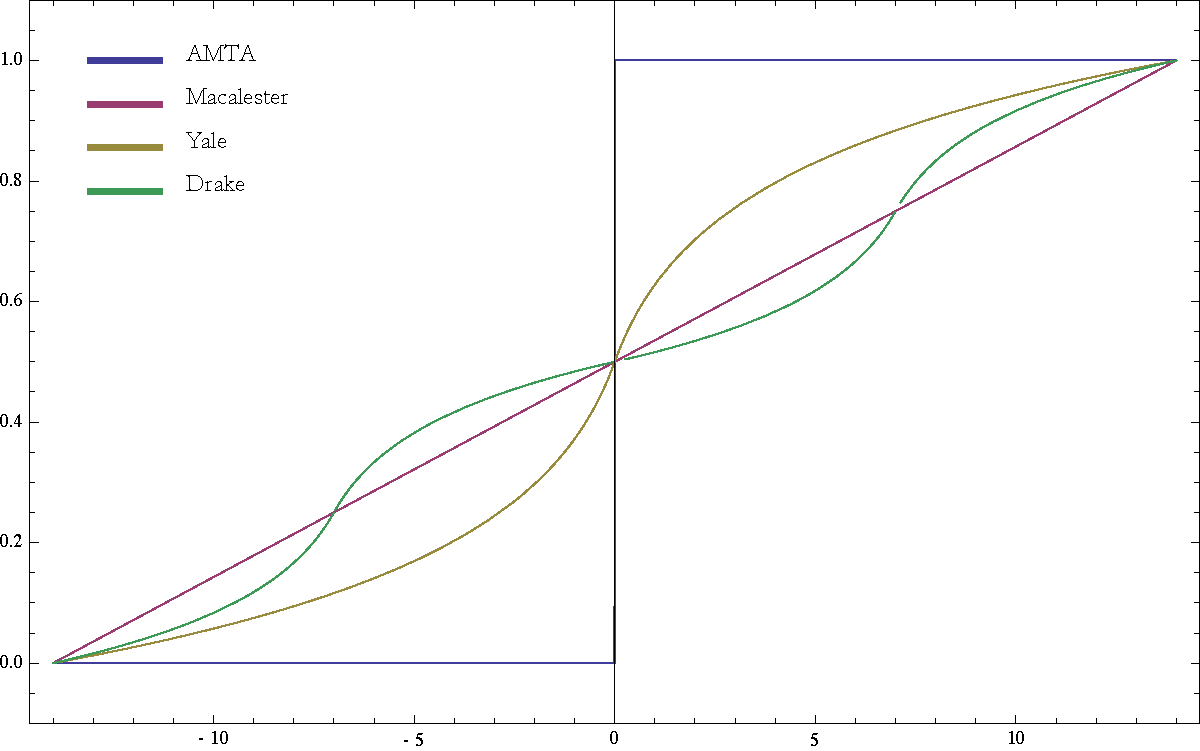
\includegraphics[width=1.0\linewidth]{BallotCurve.pdf}
\end{figure}
, Macalester uses a a straight line (Figure \ref{ballotCurves}-Red), while Yale uses a piecewise logarithmic function consisting of two regions (Figure \ref{ballotCurves}-Yellow).  The curve used at the Richard Calkins Invitational will be a piecewise logarithmic function consisting of four regions (Figure \ref{ballotCurves}-Green).  There are several motivations for selecting such a shape.  The shape of the curve is selected to recognize that PD's close to 0 ought to be weighted similarly to a tie (in comparison to Macalester's and Yale's curves, when $|PD|<\frac{QW}{2}$ the partial ballots awarded are closer to $0.5$).  Additionally, by the time the PD becomes close to $QW$, there is a similar decrease in the slope of the curve, consistent with recognizing that at that point, the winning team deserves the vast majority of the partial ballots being awarded.  This suggests a function with a large slope near $PD=\frac{\pm QW}{2}$ and a small slope near $PD=0$ and$PD=\pm QW$ achieved by:\\
\begin{displaymath}
   PB(PD) = \left\{
     \begin{array}{lr}
       \frac{1}{2}-\frac{1}{4}\left(1+\log_{\frac{QW}{2}+1}\left(1-\left(PD+\left(\frac{QW}{2}\right)\right)\right)\right) &  -QW\le x\le \frac{-QW}{2}\\
       \frac{1}{2}-\frac{1}{4}\left(1-\log_{\frac{QW}{2}+1}\left(1+\left(PD+\left(\frac{QW}{2}\right)\right)\right)\right) &  \frac{-QW}{2}<x\le 0\\
       \frac{1}{2}+\frac{1}{4}\left(1-\log_{\frac{QW}{2}+1}\left(1-\left(PD-\left(\frac{QW}{2}\right)\right)\right)\right) &  0<x\le\frac{QW}{2}\\
       \frac{1}{2}+\frac{1}{4}\left(1+\log_{\frac{QW}{2}+1}\left(1+\left(PD-\left(\frac{QW}{2}\right)\right)\right)\right) & \frac{QW}{2}\le x \le QW
     \end{array}
  \right)
\end{displaymath}
\subsection{Balancing Ballots}
\label{balancingBallots}
The second component of the partial ballot scale is selecting the endpoints constituting a QW.  To the best of my knowledge, every tournament that has employed WPB in the past has defined $QW=14$.  The argument in favor of this selection is typically that $PD=14$ indicates that the victor scored (on average) higher by $1$ on each part scored on the ballot.  While this is a reasonable approach, it is also somewhat arbitrary, in that $2$ points per part or $\frac{1}{2}$ a point per ballot are also reasonable benchmarks for saying that a team deserves to win the entire ballot.

BWPB does not seek to remove this arbitrariness, but it does raise a very closely related question:  why should the quality win be the same for both sides?  This makes sense if a case is well-balanced, however, no case is perfectly balanced, and even a case that may be be balanced in the aggregate of all tournaments may be unbalanced due to judge preferences at a particular tournament.

To address this concern, BWPB introduces a term to account for judge bias in side preference.  BWPB begins by assuming a base QW, like regular WPB (arbitrarily taken to be $14$ as is standard when using WPB).  If a case is perfectly balanced (in a given tournament, an equal number of prosecution and defense ballots are won) this QW is used for both the prosecution and the defense.  If, however, there is an imbalance in the case, each side's QW is adjusted accordingly.  Thus, for example, if out of the twenty four ballots from round 1, 16 are won by the plaintiff and 8 are won by the defense, then the plaintiff must win their ballot by $18$ points to have a complete win (because it is significantly easier to win on the plaintiff side) and the defense must only win their ballot by $9$ points for a complete win (because it is significantly harder to win on the defense side).  This balancing is cumulative, so a quality win in round 2 is determined by the balance of both the round 1 and round 2 ballots, the quality win of round 3 is determined by rounds 1, 2, and 3, et cetera\footnote{This has the interesting effect that a team's total BWPB may go down from one round to another, as the value of a prior round's ballots may go down as the case balance of the tournament changes.}.  Contrariwise, if the teams lose, the plaintiff receives no ballots if they lose by more than $-9$ points (again because it is easier to win on the plaintiff) while the defense receives a partial ballot even to scores of $-18$ points (because it is difficult to win on the defense)\footnote{It is worth pointing out that the scoring formulas are designed such that the total of partial ballot fraction awarded to each side equals $1$.  In this example, if the plaintiff has lost by $-9$ that necessitates that the defense has won by $9$, and the plaintiff receives $0$ partial ballots while the defense receives $1$.  On the other side, only if the plaintiff has won by $18$ (meaning the defense has lost by $18$) does the plaintiff receive $1$ partial ballot, while the defense receives $0$.}.  A sample set of curves appears in figure \ref{balancingCurve}.  The specific formula for calculating the plaintiff quality win (PQW) and defense quality win (DQW) are:

$PQW=2QW\left(\frac{ProsecutionBallotsWon+\frac{TiedBallots}{2}}{TotalBallots}\right)$

$DQW=2QW\left(\frac{DefenseBallotsWon+\frac{TiedBallots}{2}}{TotalBallots}\right)$

\begin{figure}[h]
\begin{center}
\label{balancingCurve}
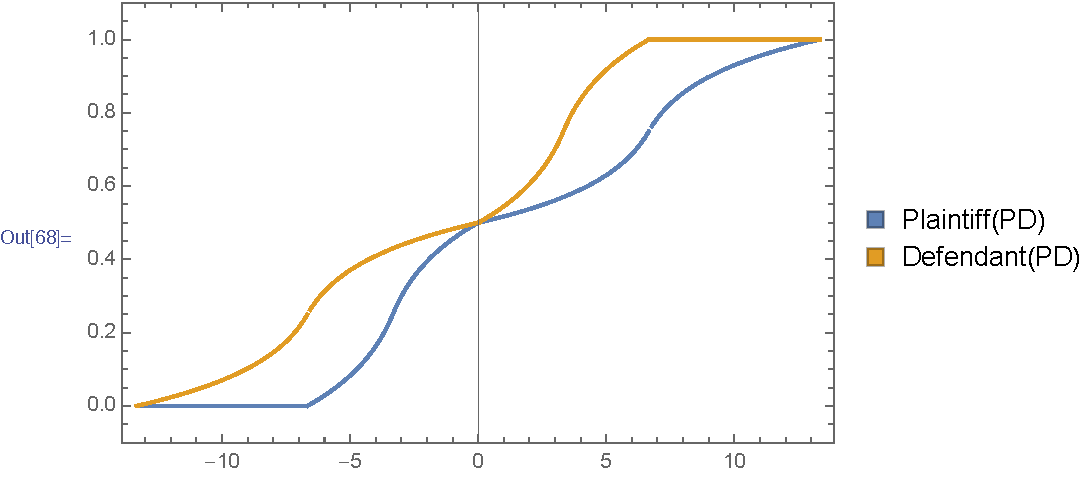
\includegraphics{BalancingCurve}
\caption{Quality win curves where the plaintiff (red) has won 16 ballots and the defense (blue) has won 8 ballots}
\end{center}
\end{figure}

\subsection{Weighted Ballots}
The final component of BWPB is the weighting of ballots in proportion to the difficulty of the team faced.  Traditional ATMA tabulation uses the opponent's strength only as a tie breaker; a team that goes 8-0 against mediocre teams places better than a team that goes 7-1 against top teams.  Like regular WPB, BWPB seeks to reward teams for victories over more difficult opponents with correspondingly more ballots when compared to a weaker opponent.  To this end, an opponent's total partial ballots factors in to calculating the total number of \textbf{weighted} ballots a team wins in a round, resulting in higher weighted ballots when facing a more difficult opponent.  The formula for the number of weighted ballots won from each partial ballot is:
\begin{center}
$WB=PB\left(OpponentsTotalPartialBallots+2\right)$
\end{center}

Each ballot's weighted ballot value is then summed together to get the total number of weighted ballots a team has won.  There are two things to note about this formula.  First, how the opponent's strength is factored into the calculation.  This is achieved by multiplying the partial ballots by the opponent's strength.  By definition, the average partial ballot value will be the number of rounds completed.  Teams that do above average (in terms of winning by more points) will have a higher number of partial ballots, while teams that do below average will have a lower number of partial ballots.  When an above average team, therefore, is an opponent (say of team 1985), this leads to multiplying team 1985's ballots by a higher value, while facing a below average team results in team 1985's partial ballots being multiplied by a lower value, thus achieving the effect of weighted ballots being sensitive to opponent's strength.

Second, there is a boost of $2$ added to the calculated amount of partial ballots prior to multiplication by the opponent's total partial ballots.  This is performed to further incentivize teams to win rounds by as much as possible as opposed to tying the round.  Without this factor, teams maximize their scores by tying ballots\footnote{$\left(.5PB\right)\left(.5OPB\right)$ is the maximum product of any two numbers whose sum equals $1$, by changing the formula to $PB\left(OPB+2\right)$ it is maximized when $PB=1$ and $OPB=0$}.  By adding the $2$ (equal to the number of judges per round), teams maximize their weighted ballots by earning a complete win as opposed to tying.\footnote{Some readers may note that the 2 additional ballots present in WPB outside of the PB product (at least as utilized at the Yale Invitational) are absent.  This is an intentional, though entirely optional removal.  Adding $2$ ballots to each weighted ballot serves no purpose in calculations for placement or pairing of teams.  While it does increase total WPB so that the sum is higher (and therefore not entirely a fraction in some early rounds), because WPB are increased by $2$ across the board, adding this factor (or removing) has no affect on placement or pairing.  As a result, for simplicity it has been removed from calculations.}
\section{Pairing Rounds}
\label{roundPairing}
\subsection{Round 1}
Round 1 at the Richard Calkins Invitational utilizes a challenge format.  Teams are first ranked using a formula dictated by the tabulation director\footnote{Factors considered in the formula include past placement at the Richard Calkins Invitational, distance travelled, and AMTA power ranking.}, with all Drake Teams automatically being ranked last with the exception of the bye-buster team, if one is required.  This formula and each team's calculated rank (and therefore challenge position) will be emailed out to all teams attending no later than the Monday prior the the Richard Calkins Invitational.

Beginning with the top ranked team, each team shall select an opponent for round 1 from the teams that have not yet selected an opponent nor been selected as an opponent.  No team may pass on their challenge.  The team being challenged shall elect to go either plaintiff or defense in round 1.  Teams may not challenge another team from their own school.  Should a team elect to challenge the bye-buster team, bye-buster's side will be determined by coin flip, with heads being bye-buster goes plaintiff and tails being bye-buster goes defense.  Due to the potential for school conflicts toward the end of the challenge draw, the tabulation director reserves the right to assign teams and sides to the extent necessary to prevent conflicts.
\subsection{Round 2}
After the calculations of partial ballots of round 1 are complete for all teams, round 2 may be paired.  \textbf{It is not necessary to calculate weighted ballots for round 2; they are not used for round 2 pairing\footnote{Partial ballots are used because using weighted ballots for rankings would add no additional information no already contained in the partial ballot ranking.  As weighted ballots are weighted by opponent strength, and after round 1 each team has had only 1 opponent, weighted ballots will merely be inversely proportional to the opponents partial ballots.  For a more thorough discussion see Graham and Wang's ``A System of Weighted Partial Ballots''.}.}  Teams that competed on the plaintiff side round 1 must go defense round 2, and teams that competed on the defense side must go on the plaintiff side round 2.  After sorting all teams into the groups of ``Needs Defense'' and ``Needs Plaintiff'', each groups' members are ranked within the groups from most partial ballots won to least partial ballots won.  In the (extremely unlikely) event that two teams have precisely the same number of partial ballots, the tie is to be broken first with the team having won more ballots (in the traditional sense) being ranked higher, then by higher point differential, then by team number as outlined in section \ref{tiebreaking}.  Once all the teams have been ranked, they are paired such that the first ranked ``Needs Plaintiff'' faces the first ranked ``Needs Defense'', et cetera.  Any impermissible matches are then resolving according to section \ref{impermissible}, resulting in the final pairings for round 2.
\subsection{Round 3}
Round 3 pairings should take place after weighted ballot calculations have been completed for all teams for round 1 and round 2.  All teams at the tournament are ranked according to the number of BWPB won.  Rank 1 faces rank 2, rank 3 faces rank 4, et cetera.  Any ties shall be broken first by number of partial ballots won, then by number of ballots won (in the traditional sense), then by the sum of the opponents' partial ballots, then by point differential, then by team number as outlined in section \ref{tiebreaking}.  Once all the teams have been ranked, any impermissible matches are resolved according to section \ref{impermissible}.  Finally, the higher ranked team in each round is assigned to the side that has won \textit{less} ballots at the tournament.\footnote{Those familiar with SAT will note that this differs from the method of round 3 side assignment used at most tournaments.  Assigning the higher ranked team the weaker side assists in distinguishing top teams that win round $3$ in spite of being on the weaker side.}  In the event that the teams are equally ranked, the ranking is determined pursuant to section \ref{tiebreaking}.
\subsection{Round 4}
Round 4 pairings should take place after weighted ballot calculations have been completed for all teams for rounds 1, 2, and 3.  Teams are sorted into two groups, ``Needs Plaintiff'' and ``Needs Defense'', and ranked by BWPB won within each group.  Tie-breaking is preformed in the same order as round 3.  Once all ties have been resolved, any impermissible matches are resolved according to section \ref{impermissible}, resulting in the final pairings for round 4.
\section{Final Placement}
After the conclusion of round 4, each teams total BWPB should be calculated.  Teams final rankings are determined by ranking them according to BWPB.  Ties are broken first by number of partial ballots won, then by number of ballots won (in the traditional sense), then by the sum of the opponents' partial ballots, then by BWPB, taking away each teams most favorable and least favorable ballot, and then by a consecutive removal process, until just 1 BWPB remains, and then by coin flip, with the lower team number ranking better if heads and the higher team number ranking better if tails.
\section{Ballot Handling Procedures}
At each captains meeting, the plaintiff team will be given two sets of ballots.  These ballots are to be filled out according to the AMTA Rulebook and Tabulation Manual policies prior to the start of the round and set in place for the judges.  Judges will be instructed on how to fill out ballots at the judge's meeting 30 minutes prior to each round.  After closing arguments, judges should give both the comment sheets and blue ballots to the timekeepers, who shall then take them to the tabulation room.
\subsection{Checking In Ballots}
Upon arriving at the tab room, timekeepers should give the blue ballots to a tabulation room representative to review to ensure that all scores have been properly recorded and all scores are legible.  If any scores or rankings are missing or illegible, the blue ballot will be sent back for clarification by the judge.  If everything is complete, both the comment sheets and blue ballots will be collected for tabulation.  \textbf{The tabulation room will not be responsible for teams not receiving ballots or comments for failure to put team numbers on ALL sheets.}
\subsection{Tabulating Ballots}
Once the ballots have been turned over to the tabulation room, comment sheets will be reviewed to determine \textit{in the aggregate only} the frequency of witness call.  Comment sheets will then be separated and filed in each team's ballot envelope.  The point differential of each blue ballot will be calculated twice, once by two different individuals.  In the event of a discrepancy, both parties will recalculate the point differential until an agreement is reached.
\subsection{Data Entry}
As BWPB uses a multi-variable logarithmic function to determine the number of ballots won, calculations of PB and BWPB are performed by a LibreOffice Sheets spreadsheet.  This spreadsheet will be emailed for review for accuracy of the formulas prior to the Richard Calkins Invitational.  Further, two different individuals on two different computers will each enter data for BWPB calculation, and compare results to prevent any data entry error.  Finally, after each round has been paired, each team has 30 minutes to have one member to review the data entry and pairings.
\section{Miscellaneous Tab Room Policies}
\subsection{Resolving Impermissible Matches}
\label{impermissible}
A team pairing is impermissible if it meets either of the following criteria:  a team facing another team from the same school or a team facing a team they have faced previously at this year's Richard Calkins Invitational.  In the event such an impermissible match occurs, it must be resolved pursuant to pages $29$-$31$ of the AMTA Tabulation Manual.  In resolving pairings, least difference is determined first by BWPB (except for round 2), then by PB, then by ballots won, then by opponent's total PB, then by CS, then by PD.
\subsection{Team Number Tie-Breaking}
\label{tiebreaking}
In the event that teams are tied for rankings when pairing a round such that the tie cannot be resolved by policies stated in section \ref{roundPairing}, the tie is to be resolved by coin flip.  For that particular tie, the teams are ranked with the lowest team number being first and the highest being last, contrariwise if the coin flip is tails.  This procedure is repeated for each individual tie, that is to say, each tie will have its own individual coin flip.
\subsection{Drops}
Should a team drop from the tournament, that team loses all eligibility for team awards or individual awards.  For the purpose of calculating that team's opponents' weighted partial ballots, it shall be assumed that the dropping team would continue to received the amount of partial ballots they received in the rounds they were present for.  Thus a team (suppose 1985) dropping after round 2 would have partial ballots from round 1 and round 2.  When calculating their opponents' weighted partial ballots for round 3, team 1985's partial ballots would be multiplied by $1.5$ and when calculating for round 4, they would be multiplied by $2$.
\subsection{Bye-Buster Teams}
In the event that there is a bye-buster team, there are two notable exceptions to the polices outlined elsewhere in this tabulation manual.  First, the bye-buster is always ranked last for pairings, regardless of performance.  Second, the bye-buster team, if challenged, has its side selected by coin flip.
\subsection{Individual Awards}
The Richard Calkins Invitational anticipates awarding individual awards roughly equal to half the number of teams attending for attorneys and witnesses.  These values may change depending on the number of ranks awarded.  Judges are required to rank at least two attorneys and two witnesses in each round.  They are encouraged, but not required to rank four.  Reasonable minds may differ as to whether judges should be required to complete all four ranks.  On the one hand, failing to require rankings may lead to judges that do not rank any individuals at all.  On the other hand, requiring judges to rank four individuals, even when they feel that there were not four outstanding performers, may artificially increase the number of ranks necessary for individuals to receive awards.  In light of these considerations, this year the Richard Calkins Invitational will require at least two individuals ranks with the option to include up to four.
\subsection{Availability of Tabulation Information}
The tabulation room will be open from the beginning of the tournament until the first set of ballots from round $4$ is turned in for tabulation.  After that point, only members of Drake Mock Trial and other individuals approved by the tournament board or tabulation director will be permitted in the tabulation room.  We also recognize that due to the reliance on computerized calculations to determined BWPB, teams may wish to review the spreadsheet throughout the tournament.  The tabulation room will have several computers setup specifically for review use.  Additionally, a link to the spreadsheet will be emailed \textbf{to the coach or designated contact person of each team} after each round's tabulation is complete (except for round $4$).  It is \textbf{your} responsibility to prevent other members of your program from accessing this file if you do not wish it.  Finally, case balance information, as well as what PD constitutes a QW for each side will be posted in the tabulation room, and is also included on the tabulation summary spreadsheet.
\subsection{Interpretation/Changes}
The tabulation director (as author of this manual) has the authority to interpret this manual as he sees fit, and to depart from the policies outlined herein as may be necessary for the smooth and expedient operation of the tournament.
\section{Acknowledgments}
The ideas in this manual were heavily influenced by those found in ``A System of Weighted Partial Ballots'' by Graham and Wang.  Additional inspiration came from a review of the Macalester Trials tabulation summary supplement.  Thank you to Zach Valentine of Iowa State University and Cecilia Panella, Kian Stack, and Natalie Hedberg of Drake University for their comments as well.
\end{document}